% Copyright (C) 2013 Thomas L. Kula
% All Rights Reserved
%
% See the file LICENSE for license terms.
\documentclass[12pt]{article}
\usepackage{graphicx}
\usepackage{rotating}
\usepackage{fix-cm}
\usepackage{multirow}
\setlength{\paperwidth}{5.5in}
\setlength{\paperheight}{8.5in}
\setlength{\textheight}{7.45in}
\setlength{\topmargin}{-1.0in}
\setlength{\oddsidemargin}{-0.5in}
\setlength{\evensidemargin}{-0.5in}
\setlength{\textwidth}{4.0in}
\setlength{\parindent}{0in}
\setlength{\parskip}{3mm}
\usepackage[print]{booklet} \nofiles
\source{\magstep0}{5.5in}{8.5in}
\target{\magstep0}{11in}{8.5in}
\setpdftargetpages
\pagestyle{empty}
\begin{document}


\begin{center}
{\fontsize{36}{48}\selectfont \textsc{Haiku a Day }}
\end{center}

\vspace*{3.5cm}

{\fontsize{20}{40}\selectfont 

Let the rays go down

Let the day time end sooner

Winter brings night time

}

\vspace*{5.0cm}
\begin{center}
{\large{Issue 98: August 2013}} \\[5mm]
{\fontsize{8}{8}\selectfont  \textsc{ St. Joshua Norton Press }} \\[1mm]
{\fontsize{6}{6}\selectfont Mathom House by the Cloisters \textbar The People's Republic of Ames }
\end{center}


\newpage

It's fitting that when I finally get around to putting the August issue
together, we're getting a mini-summer here in NYC.

--- Thomas

http://kula.tproa.net/had/ \\
kula@tproa.net

Download this and previous HADs at the website, so you can
print out your own (DIY, yeah!) or if you want me to send
you one, send me your address, and maybe a stamp if you
are feeling nice. Or send me something you've made ---
trades always appreciated, postcards are nice too.

\vfill

1 August 2013

With a grinding POP! \\
The blender gives up the ghost \\
To a better place

2 August 2013

Your sheets are cotton \\
Simple, white, and with no fuss \\
Anything else pales

3 August 2013

A subway ride away \\
An awesome band is playing \\
There on the platform

\newpage

4 August 2013

A bumbling robot \\
May be more useful than this \\
Crappy help system

5 August 2013

Hunger the best sauce \\
Or at least hallucogen \\
PB-Cheerios

6 August 2013

Flags change direction \\
The scent of the air, subtle \\
Becomes sea salty

7 August 2013

A friend off for years \\
A whole evening of dinner \\
And of catching up

8 August 2013

A combat gymnast \\
Second Pommel Horse Brigade \\
Jumps in formation

9 August 2013

Aquatic pounding \\
The river, running high, spills \\
The drains do not hold

10 August 2013

A beautiful night \\
Gorgeous park, favorite band \\
I love living here

\newpage
11 August 2013

A pile of kale \\
Sauted, sesame oil \\
Food for the whole week

12 August 2013

Distant cargo floats \\
Grabbed by the sky, it settles \\
One more ride then home

13 August 2013

On a pedestal \\
You have greater potential \\
Do not squander it

14 August 2013

A hungry city \\
Somehow swallowed up my phone \\
Glad for insurance

15 August 2013

Waiting for a phone \\
As the clock ticks, time slows down \\
Call me when its here

16 August 2013

An evening, empty \\
Countless possibilities \\
Should I stay or go?

17 August 2013

Monochromatic \\
The first light of dawn breaking \\
Pale hint of the day

\newpage
18 August 2013

Data injustice \\
File strewn about the place \\
Clean out the homedir

19 August 2013

The front of the train \\
Flying off into the sky \\
Dawn, the aqueduct

20 August 2013

In a pinch, fake it \\
You'll probably get away \\
There's nothing to lose

21 August 2013

Victory, defeat \\
Sometimes things are both of them \\
Life is not simple

22 August 2013

Fair distribution \\
A bit here, and a bit there \\
Good, but not much fun

23 August 2013

A low triangle \\
Watches the traffic go by \\
Sitting, biding time

24 August 2013

Fire a privilege \\
Use its power carefully \\
Or you will get burned

\newpage

25 August 2013

A solid dresser \\
Does not move that easily \\
Short pain for long life

26 August 2013

It is not painless \\
But a complete scrubbing gives \\
Joy beyond belief 

27 August 2013

A siren, drawling \\
Lazily asks, move aside \\
Slacker firetruck

28 August 2013

Getting in my way \\
Swarms of students move slowly \\
Blocking the sidewalk

29 August 2013

Shower to get clean? \\
Or a bit of a reprieve, \\
From the day ahead?

30 August 2013

In a raven's claw \\
The head of the poet Poe. \\
``You say nevermore!"

31 August 2013

Doctor Octopus \\
Operates two at a time \\
Tentacles to spare

\newpage

\begin{center}
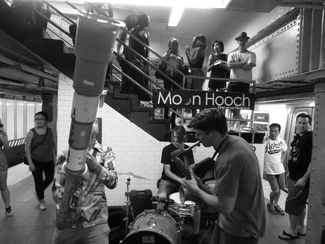
\includegraphics[width=325pt]{moon-hooch.png}
Moon Hooch at the 14th Street/Union Square L Stop \\
3 August 2013 \\
{\tt kula.tproa.net/photos/2013/20130803-moonhooch }
\end{center}

\newpage

\thispagestyle{empty}
\vspace*{12cm}
\begin{sideways}
\Large{St. Joshua Norton Press}
\end{sideways}
\begin{sideways}
\Large{PO Box 250138}
\end{sideways}
\begin{sideways}
\Large{New York NY 10025}
\end{sideways}


\end{document}


